%%%%%%%%%%%%%%%%%%%%%%%%%%%%%%%%%%%%%%%%%%%%%%%%
% 1. Document class 
\documentclass[a4paper,12pt]{article} % This defines the style of your paper
%%%%%%%%%%%%%%%%%%%%%%%%%%%%%%%%%%%%%%%%%%%%%%%%
% 2. Packages
\usepackage[top = 2.5cm, bottom = 2.5cm, left = 2.5cm, right = 2.5cm]{geometry} 
\usepackage[T1]{fontenc}
\usepackage[utf8]{inputenc}
\usepackage{multirow} % Multirow is for tables with multiple rows within one cell.
\usepackage{booktabs} % For even nicer tables.
\usepackage{graphicx} 
\usepackage{setspace}
\setlength{\parindent}{0in}
\usepackage{float}
\usepackage{fancyhdr}
\usepackage{titlesec}
\usepackage{url}
\usepackage{amsmath,amssymb,amsthm,bm}
\usepackage{subcaption}
\usepackage{setspace}
\usepackage{etoolbox}
\AtBeginEnvironment{quote}{\singlespace\vspace{-\topsep}\small}
\AtEndEnvironment{quote}{\vspace{-\topsep}\endsinglespace}

\titleformat*{\section}{\large\bfseries}
\titleformat*{\subsection}{\bfseries}
%%%%%%%%%%%%%%%%%%%%%%%%%%%%%%%%%%%%%%%%%%%%%%%%
% 3. Header (and Footer)
\pagestyle{fancy} % With this command we can customize the header style.
\fancyhf{} % This makes sure we do not have other information in our header or footer.
\lhead{\footnotesize  CS 7180}% \lhead puts text in the top left corner. \footnotesize sets our font to a smaller size.
%\rhead works just like \lhead (you can also use \chead)
\rhead{\footnotesize Assignment 3} %<---- Fill in your lastnames.
% Similar commands work for the footer (\lfoot, \cfoot and \rfoot).
% We want to put our page number in the center.
\cfoot{\footnotesize \thepage}

\graphicspath{ {./imgs/} }

\begin{document}
\thispagestyle{empty} % This command disables the header on the first page. 

\begin{tabular}{p{15.5cm}} % This is a simple tabular environment to align your text nicely 
{\large \bf CS 7180 Special Topics in AI: Deep Learning} \\
Northeastern University, Spring 2019 \\
\hline % \hline produces horizontal lines.
\end{tabular} % Our tabular environment ends here.

\vspace*{0.3cm} % Now we want to add some vertical space in between the line and our title.

\begin{center} % Everything within the center environment is centered.
    {\Large \bf Assignment 3} % <---- Don't forget to put in the right number
    \vspace{2mm}
    
        % YOUR NAMES GO HERE
    {Name: Tyler Brown UID: 001684955}
\end{center} 
%
\vspace{0.2cm}

The goal of Assignment 3 is to train a generative adversarial network
that can draw sketches. My implementation is based on ``A Neural
Representation of Sketch Drawings'' \cite{DBLP:journals/corr/HaE17} by
Ha and Eck (2017). 

\section{Rendering}

Figure \ref{fig:rendersheep} contains an image of a sheep that I rendered
using the \textit{draw\_strokes.py} script provided to us in this assignment.

\begin{figure}[h]
  \begin{center}
    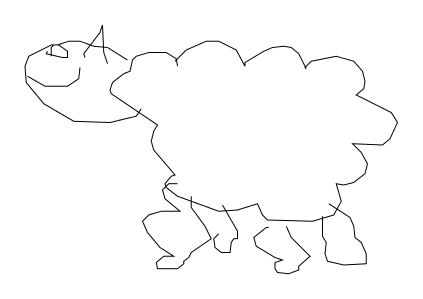
\includegraphics[scale=0.5]{sample_sheep}
    \caption{Rendering a Sheep Image}
    \label{fig:rendersheep}
    \end{center}
\end{figure}

\section{Pre-processing}

The pre-processing steps I used were very similar to those by Ha and Eck
\cite{DBLP:journals/corr/HaE17}. Alexis David Jacq, a PhD student and
intern at Google Brain, implemented the Ha and Eck model
using PyTorch \cite{alexisja77:online}. It make sense to include many of his
pre-processing steps in my model because is processing identical data.
The Ha and Eck paper \cite{DBLP:journals/corr/HaE17} is so similar that their
README file on GitHub includes the graphic used in Section 2.1 of our
Assignment 3 handout.\newline

Pre-processing steps are broken out into my \textit{SketchDataPipeline}
class in \textit{sheepgan.py}. These steps include

\begin{enumerate}
\item Finding the maximum sequence size for additional preprocessing
\item Purifying strokes to remove sequences that are too small or too long.
  It also removes large gaps.
\item Normalize the dataset by a normalizing scale factor.
\end{enumerate}

In terms of modifying Ha and Eck \cite{DBLP:journals/corr/HaE17} to be
compatible with a GAN, I added a batch generation method, and a special
type casting method for output from the generator. The batch generation
method for my GAN model randomly selects a batch of normal data, keeps
the sequence lengths and batch dimensions, then replaces all normal data
with randomly selected values within the range of values seen in normal
data. You'll also see a ``gencast\_tensor'' method which is unfortunately
where I got stuck at the deadline. This casting method reformats output from
the generator so it can be fed into the discriminator.

\section{GAN}

The GAN I chose to construct is really exciting to me because it attempted
to modify Sketch-RNN, a Sequence-to-Sequence Variational Autoencoder (VAE)
\cite{DBLP:journals/corr/HaE17}. These models are typically seen as an
opposite approach to a GAN model. Without getting into too many low level
details related to Sketch-RNN, this model allows for image generation
conditional on a batch item. If we create random data of the same dimensions
as a normal batch item, then it is feasible that sketch-rnn could be used
as a generator. Following the same idea, we can take the predicted strokes,
reprocess the output, then feed that output into a discriminator. The
discriminator can use the generator's output to conditionally generate its
own image. We could also randomly use true images.We could then use a loss
function to compute the difference between the discriminator's image and the
valid image from true data.  This loss function would update the GAN
optimizer. When sketches created by the discriminator become closer to the
valid image, then we should be able to approximate the underlying
distribution.\newline

Theoretical advantages of using a GAN on top of two Sequence-to-Sequence
VAE's may help better approximate the loss function. My understanding is
that the current loss function being used by these models is a proxy for
an intractable loss function dictated by theory. Using a GAN to bring these
approximate bounds in closer could yield better accuracy results. \newline

I was able to create several outputs with the generator. I compared those
with outputs from Jacq \cite{alexisja77:online} using a cat instead of a
sheep. His cats look better than my sheep so I'll most likely need to
revisit my hyperparameters. Figure \ref{fig:gen3500} provides an example
of a sheep conditionally generated after 3400 epochs. \newline

\begin{figure}[h]
  \begin{center}
    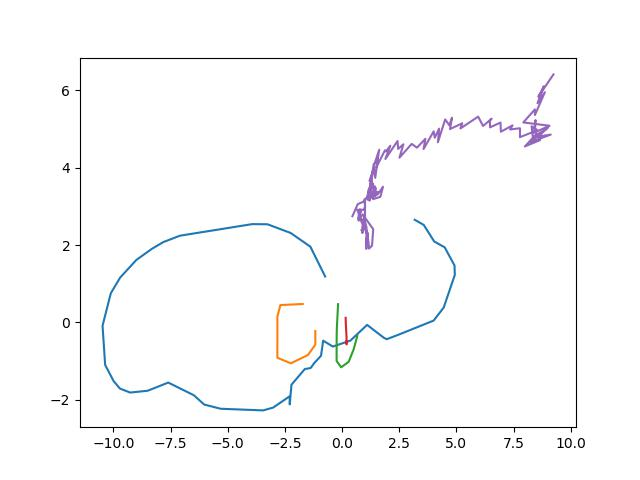
\includegraphics[scale=0.5]{3400_output_}
    \caption{Generator after 3500 Epochs using True Data}
    \label{fig:gen3500}
    \end{center}
\end{figure}

The intuition is to improve conditionally generated images from the
Sequence-to-Sequence VAE using a GAN which can help better approximate
its loss function. This intuition can be readily tested using an experiment.
We can see that I was able to get the generator working without an issue. I
was also able to get the discriminator to train independently. I had issues
getting the handoff from generator to discriminator working correctly in the
time we have available for this assignment.

\section{Improving GAN}

This GAN could be improved by debugging the dimensionality associated with
a handoff from generator to discriminator. Once this is working, additional
thought could be taken to choose a GAN loss function to best optimize this
model. We can anticipate sequences of different lengths so choosing a
loss function which is robust to these sequence length variations will require
careful thought.\newline

I was able to improve over a basic GAN implementation by modifying a
Sequence-to-Sequence VAE. I was able to get several components of this model
working but not the whole thing. In terms of modifications, I did go
through the Sequence-to-Sequence VAE and put substantial effort into
figuring out a way that it could be modified for use as a GAN.


\bibliographystyle{unsrt}
\bibliography{references}


\end{document}
